\chapter{Database Schema}
\label{ch:database-schema}

\section{Schema Overview}
\label{sec:schema-overview}

This chapter provides the complete SQL schema definition for \projectname{}, including key tables, relationships, data types, constraints, and indexes.

% ============================================
% SCHEMA DIAGRAM
% ============================================
\section{Visual Schema Diagram}
\label{sec:schema-diagram}

\begin{figure}[H]
\centering
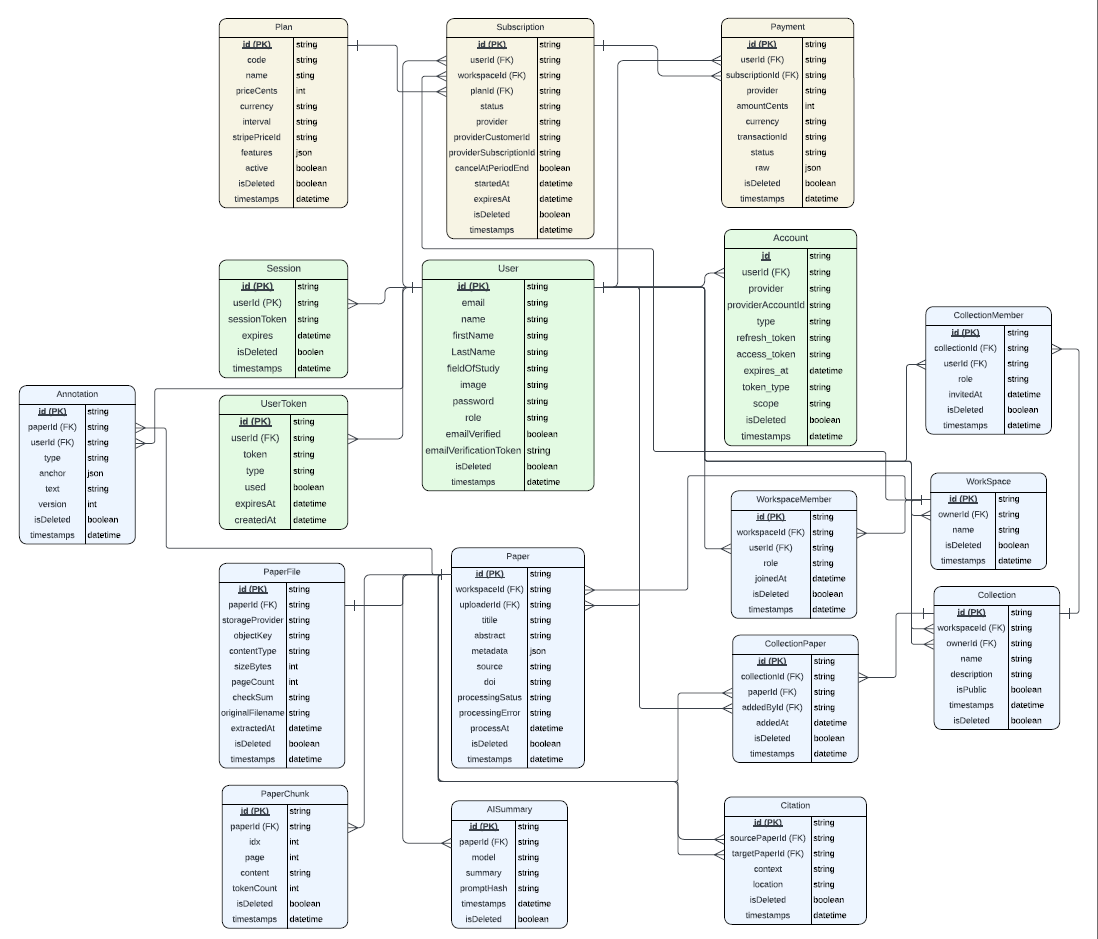
\includegraphics[width=0.95\textwidth]{images/diagrams/schema.png}
\caption{ScholarFlow Complete Database Schema}
\label{fig:schema-complete}
\end{figure}

\noindent For detailed schema view: \url{https://lucid.app/lucidchart/8fa45201-ebc1-46e2-8204-93c162cbaf0b}

% ============================================
% CORE TABLES OVERVIEW
% ============================================
\section{Core Tables Overview}
\label{sec:schema-tables-overview}

The database consists of 24 interconnected tables organized into functional modules:

\subsection{1. Authentication \& User Management}
\begin{itemize}[leftmargin=*,topsep=3pt,itemsep=2pt]
    \item \texttt{User}: User profiles with authentication credentials (email, password hash)
    \item \texttt{Account}: OAuth provider accounts linked to users (Google, GitHub)
    \item \texttt{Session}: Active user sessions with JWT tokens
    \item \texttt{VerificationToken}: Email verification and password reset tokens
\end{itemize}

\subsection{2. Paper Management}
\begin{itemize}[leftmargin=*,topsep=3pt,itemsep=2pt]
    \item \texttt{Paper}: Research papers with metadata (title, authors, abstract, publication year)
    \item \texttt{PaperFile}: File storage references (S3 URLs, file sizes, MIME types)
    \item \texttt{PaperChunk}: Text segments extracted from papers for AI processing
    \item \texttt{PaperTag}: Custom tags for categorization
\end{itemize}

\subsection{3. Collections \& Organization}
\begin{itemize}[leftmargin=*,topsep=3pt,itemsep=2pt]
    \item \texttt{Collection}: User-created collections with privacy settings
    \item \texttt{CollectionPaper}: Many-to-many relationship between collections and papers
    \item \texttt{CollectionMember}: Shared collection access with role-based permissions
\end{itemize}

\subsection{4. AI Features}
\begin{itemize}[leftmargin=*,topsep=3pt,itemsep=2pt]
    \item \texttt{AISummary}: AI-generated paper summaries
    \item \texttt{AIInsightThread}: Conversation threads about papers
    \item \texttt{AIInsightMessage}: Individual messages in AI conversations
\end{itemize}

% ============================================
% TABLE DEFINITIONS
% ============================================
\section{Core Table Definitions}
\label{sec:schema-tables}

\subsection{User Table}
\begin{lstlisting}[language=SQL, caption={User Table Schema}]
CREATE TABLE "User" (
  id SERIAL PRIMARY KEY,
  name VARCHAR(255),
  email VARCHAR(255) UNIQUE NOT NULL,
  emailVerified TIMESTAMP,
  image TEXT,
  password TEXT,
  role VARCHAR(50) DEFAULT 'RESEARCHER',
  bio TEXT,
  institution VARCHAR(255),
  field VARCHAR(255),
  googleScholarUrl TEXT,
  orcidUrl TEXT,
  createdAt TIMESTAMP DEFAULT NOW(),
  updatedAt TIMESTAMP DEFAULT NOW()
);

-- Indexes
CREATE UNIQUE INDEX "User_email_key" ON "User"(email);
CREATE INDEX "User_role_idx" ON "User"(role);
\end{lstlisting}

\subsection{Paper Table}
\begin{lstlisting}[language=SQL, caption={Paper Table Schema}]
CREATE TABLE "Paper" (
  id SERIAL PRIMARY KEY,
  title VARCHAR(500) NOT NULL,
  authors TEXT,
  abstract TEXT,
  publicationYear INTEGER,
  journal VARCHAR(255),
  doi VARCHAR(255),
  fileUrl TEXT NOT NULL,
  fileName VARCHAR(500) NOT NULL,
  fileSize BIGINT NOT NULL,
  fileType VARCHAR(50) NOT NULL,
  uploaderId INTEGER NOT NULL REFERENCES "User"(id),
  workspaceId INTEGER NOT NULL REFERENCES "Workspace"(id),
  isDeleted BOOLEAN DEFAULT FALSE,
  deletedAt TIMESTAMP,
  createdAt TIMESTAMP DEFAULT NOW(),
  updatedAt TIMESTAMP DEFAULT NOW()
);

-- Performance Indexes
CREATE INDEX "Paper_uploaderId_workspaceId_idx" 
  ON "Paper"(uploaderId, workspaceId);
CREATE INDEX "Paper_workspaceId_isDeleted_idx" 
  ON "Paper"(workspaceId, isDeleted);
CREATE INDEX "Paper_title_authors_gin_idx" 
  ON "Paper" USING gin(to_tsvector('english', title || ' ' || authors));
\end{lstlisting}

\subsection{Indexing Strategy}
\begin{itemize}[leftmargin=*,topsep=3pt,itemsep=2pt]
    \item \textbf{Unique Indexes}: \texttt{User.email}, \texttt{Account.(provider, providerAccountId)}
    \item \textbf{Foreign Key Indexes}: All foreign key columns for efficient joins
    \item \textbf{Composite Indexes}: \texttt{(workspaceId, uploaderId)}, \texttt{(collectionId, paperId)}
    \item \textbf{Full-Text Indexes}: \texttt{Paper.title}, \texttt{Paper.abstract} for search
    \item \textbf{Timestamp Indexes}: \texttt{createdAt} columns for chronological queries
\end{itemize}

% ============================================
% COMPLETE SCHEMA
% ============================================
\section{Complete Schema SQL}
\label{sec:schema-complete-sql}

\begin{infobox}[Full Schema]
The complete schema includes 24 tables with all relationships. For the full Prisma schema definition, see:

	exttt{apps/backend/prisma/schema.prisma}

Or generate SQL:
\begin{lstlisting}[language=bash]
yarn db:migrate dev --name schema_export
\end{lstlisting}
\end{infobox}
